\documentclass[12pt, a4paper, twoside]{article}

\usepackage{tex/style/snowrake}
\usepackage{amsmath, bm, tikz, subfig, nicematrix, amssymb, csquotes, diffcoeff}
\usepackage[framemethod=tikz]{mdframed}

\author{Gábor Szijártó}
\title{Sample Standard Deviation Explained}
\date{}
\renewcommand{\srcompany}{Medium}
\renewcommand{\srtitle}{}
\renewcommand{\srdocver}{v0}
\newcommand{\mat}[1]{\bm{#1}}
%\captionsetup[subfigure]{labelformat=empty}

\DeclareMathOperator{\srexpop}{\mathbb{E}}
\DeclareMathOperator{\srexvar}{\mathbb{V}}
\newcommand\srexp[1]{\srexpop\left[#1\right]}
\newcommand\srvar[1]{\srexvar\left[#1\right]}
\definecolor{backquote}{RGB}{224,215,188}
\mdfdefinestyle{srquotesty}{hidealllines=true, roundcorner=5pt, backgroundcolor=backquote!30}

\begin{document}

\srdocsimple

Statistics is a must have for any ML/DL engineer and data scientist!\\
In this article I will cover a simple yet interesting equation: \textbf{Sample Standard Deviation}\\

\begin{equation}
	s^2 = \frac{\sum_{i=1}^{n}(x_i - \bar{x})^2}{n - 1}
\end{equation}

This is the equation for the \textbf{unbiased sample variance}.\\
Why is it called 'unbiased' and why do we have $n-1$ term in the denominator?\\
These are the questions that will be answered.


\subsection*{Bessel's Correction}

A commonly used intuitive explanation is the  \href{https://en.wikipedia.org/wiki/Bessel\%27s\_correction#Source\_of\_bias}{Bessel's correction}.

\begin{displayquote}
\begin{mdframed}[style=srquotesty]
\enquote{While there are n independent observations in the sample, there are only\\ n - 1 independent residuals, as they sum to 0}
\end{mdframed}
\end{displayquote}

It states that we need to use n-1 as there are only n-1 independent variables, because the expected value is calculated based on the samples. In case we have n-1 degree of freedom, then it makes sense to divide by $n-1$ instead of n.\\

Easy to grab explanation, but I feel it kind of confusing and misses the most important point, the real reason behind the need for correction!\\

Why do I think it can be confusing?\\
Let's calculate the standard deviation of a uniform discrete random variable like 6 sided fair dice.

\begin{equation}
	\sigma^2 = \srvar{X} = \frac{\sum_{i=1}^{N}(x_i - \mu)^2}{N}
\end{equation}

The expected value is not independent from the possible values as it can't be by its definition, yet we are dividing
by $N$ instead of $N -1$.

\begin{gather*}
	\mu = \srexp{X} = \sum_{i=1}^{6}\frac{1}{6}x_i = 3.5\\[1em]
	\srvar{X} = \frac{\sum_{i=1}^{6}(x_i - \mu)^2}{6} \approx 2.9166
\end{gather*}

It can be confusing.


\subsection*{Understanding the Need for Correction}

Understanding the essence behind the correction will immediately reveal why we need to divide by
$n$ in some applications and by $n-1$ in others.\\

The major difference between sampling from a population and knowing all elements of it or the distribution itself, is that in the latter case we know the exact value of $\mu$, while in case of sampling we have only an estimate of it.\\
\textbf{To be able to calculate the variance we must know the real $\mu$, not just an estimation.}\\
The error of estimated expected value induces a bias into the variance calculations!

\begin{gather*}
	\mu = \text{real expected value of the population} \\[1em]
	\bar{X} = \srexp{X} = \text{calculated expected value value based on sample} \\[1em]
	\srvar{X} = \srexp{(X - \mu)^2} \neq \srexp{(X - \bar{X})^2}
\end{gather*}

We divide $n-1$ instead of $n$ to get an unbiased estimation for the population's variance!\\
Can we prove it? Yes, only a small idea needs to be applied.

\begin{figure}[H]
\centering
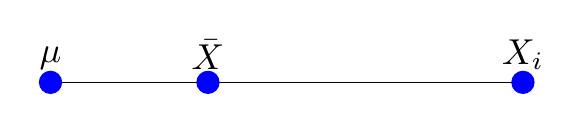
\begin{tikzpicture}[scale=2, every node/.style={scale=1.3}]
	\coordinate (mu) at (0,0);
	\coordinate (xbar) at (1,0);
	\coordinate (x) at (3,0);

	\draw[-] (mu) -- (xbar);
	\draw[-] (xbar) -- (x);
	\filldraw[draw=blue, fill=blue] (mu) circle (2pt) node[anchor=south] {$\mu$};
	\filldraw[draw=blue, fill=blue] (xbar) circle (2pt) node[anchor=south] {$\bar{X}$};
	\filldraw[draw=blue, fill=blue] (x) circle (2pt) node[anchor=south] {$X_i$};
\end{tikzpicture}
\end{figure}

\begin{equation}
	X_i - \mu = (\bar{X} - \mu) + (X_i - \bar{X})
\end{equation}

Lets substitute equation (3) into (2).

\begin{gather*}
	\sigma^2 = \srvar{X} = \srexp{(X - \mu)^2} = \srexp{ \left((\bar{X} - \mu) + (X - \bar{X})\right)^2} \\[1em]
	= \srexp{(\bar{X} - \mu)^2} + 2 \srexp{(\bar{X} - \mu) (X - \bar{X})} + \srexp{(X - \bar{X})^2} \\[1em]
	= \srvar{\bar{X}} + 2 (\bar{X} - \mu) \srexp{X - \bar{X}} + \srexp{(X - \bar{X})^2}
\end{gather*}

Evaluating the terms separately:

\begin{equation}
	\srvar{\bar{X}} = \srvar{\frac{\sum{X}}{n}} = \frac{1}{n^2}\srvar{\sum{X}} = \frac{1}{n^2}\sum\srvar{X} = \frac{\srvar{X}}{n} = \frac{\sigma^2}{n}
\end{equation}
The assumption that variables are \textbf{independent} was used here!\\
This is true only in the case we are sampling with replacement, so the same element is allowed to be sampled multiple times!

\begin{equation}
	\srexp{X - \bar{X}} = \srexp{X} - \bar{X} = 0
\end{equation}
This makes the whole middle term zero!

\begin{equation}
	\srexp{(X - \bar{X})^2} = \srexp{(X - \srexp{X})^2} = \sigma_s^2
\end{equation}
By the definition of variance.\\
In the calculations above basic properties of the expected value and variance were used.

Substitute back the results of (4, 5, 6)!
\begin{align*}
	\sigma^2 &= \frac{\sigma^2}{n} + 0 + \sigma_s^2 \\[1em]
	\sigma^2 &= \frac{n}{n-1} \sigma_s^2 
\end{align*}

$\frac{n}{n-1}$ is the correction term applied to get an unbiased estimator for population variance.\\[1em]
This results in the well known equation:

\begin{equation}
	\mathbf{\sigma^2} = \frac{n}{n-1} \sigma_s^2 = \frac{n}{n-1} \frac{\sum_{i=1}^{n}(x_i - \bar{x})^2}{n} = \mathbf{\frac{\sum_{i=1}^{n}(x_i - \bar{x})^2}{n - 1}}
\end{equation}
\\[1em]
Since $\frac{n}{n-1}$ is greater than $1$, we can conclude that $\sigma_{s}$ \textbf{underestimates} the true sample variance.\\
As the number of samples increases, $\sigma_{s}$ will converge to $\sigma$.

%\subsection*{Sample Variance Minimum when Unbiased}

%We reached the conclusion that we are underestimating the variance by a factor of $\frac{n-1}{n}$.\\
%We will prove that a sample's variance is minimum in case it is calculated based on the sample's mean.

%\begin{equation*}
	%\min{ f(a) } = \frac{\sum_{i=1}^{n}(x_i - a)^2}{n}
%\end{equation*}

%Check when the derivative becomes zero, it will be the minimum.
%\begin{align*}
%	\diffp{\sum_{i=1}^{n}(x_i - a)^2}a &= 0 \\[1em]
%	\diffp{\sum{\left( x^2 - 2ax + a^2\right)}}a &= 0 \\[1em]
%	-2 \sum x + 2 \sum a &= 0 \\[1em]
%	2na &= 2\sum x \\[1em]
%	a = \frac{\sum x}{n} &= \bar{x}
%\end{align*}

\end{document}
